\chapter{Simmetrie}

Riprendiamo la discussione sulle simmetrie introdotta nella sezione \ref{sec: sim_intro}. 
Espandiamo il concetto di simmetria da un semplice cambio di visuale a vere e proprie trasformazioni di stati e osservabili, che mantengano sempre invariati i valori medi:
\begin{equation}
    \Sigma\to \Sigma' \qquad \mathcal{A}\to \mathcal{A}' \qquad  \text{ t.c. } \expval{\mathcal{A}}_\Sigma  = \expval{\mathcal{A}'}_\Sigma
\end{equation}

Dal teorema di Wigner \ref{theo: Wigner} sappiamo che queste trasformazioni \(\tau\) sono indotte da operatori unitari o antiunitari \(U\), ma il teorema non garantisce l'unicità dell'operatore per simmetria.

\begin{theorem}
    Due operatori unitari o antiunitari \(U, \ U'\) inducono la stessa simmetria se e solo se \(U ' = e^{i\theta}U\) .
\end{theorem}
\begin{proof}
    \((\impliedby) \) 
    \[
        \left[ \Psi \right]\to \left[ e^{i\theta}U \Psi\right]= \left[ \Psi \right] \quad A \to e^{i\theta}UAU^\dagger e ^{-i\theta}= UAU^\dagger
    \]
    \((\implies) \) supposto che \(\tau_U = \tau_{U'}: \ \ UAU^\dagger = U'AU'^\dagger\) abbiamo che:
    \[
       U^\dagger U A U^\dagger U'= U^\dagger U'A A'^\dagger U'  \implies AU^\dagger U'= U^\dagger U ' A
       \implies \left[ U^\dagger U', A \right]=0
    \] 
    Sfruttiamo il lemma: \(B\) t.c. \(\left[ B,A \right]= 0 , \ A \) a.a. \(\implies B = \lambda I\).
    \[
        \implies U^\dagger U' = \lambda I , \ \abs{\lambda} = 1 \implies U ' = e^{i\theta}U
    \]
\end{proof}
Perciò ogni trasformazione di simmetria \(\tau\) è indotta da un \textit{raggio operatore} (anti)unitario:
\begin{equation}
    \left[ U_\tau \right]= \left\{ U \ \text{ (anti)unitario t.c. } U' = e^{i\theta}U , \ \theta \in \mathbb{R}\right\}
\end{equation}

\begin{remark}
    \(I\) è simmetria, composizione di simmetrie \(\tau_1 \circ \tau_2\) è simmetria e \(\tau^{-1}\) è simmetria.
\end{remark}


\section{Gruppo di simmetria}
\begin{definition}
    Definiamo \textit{gruppo} \((G; \cdot )\) un insieme \(G\) dotato di un'operazione \(\cdot \) :
    \begin{equation}
        \cdot : G \times G \to G \qquad (g,h)\to gh
    \end{equation}
    tale che:
    \begin{itemize}
        \item Associativa: \((gh)k= g(hk) \quad \forall\, g,h,k \in G\) .
        \item Esiste neutro: \(\exists 1 \in G :\ 1g = g1 = g \quad \forall \, g \in G\) .
        \item Esiste inverso: \(\forall \, g \in G , \ \exists\, g^{-1}\in G : \ gg^{-1}= 1 = g^{1}g\)
    \end{itemize}
\end{definition}
Se vale anche la proprietà commutativa \(gh = hg \ \forall\, g,h \in G\) allora il gruppo si dice \textit{abeliano}.
\begin{remark}
    Si dimostra che \(1\) e \(g^{-1}\) dato \(g\) sono unici.
\end{remark}

\begin{example}
    \((\mathbb{Z}; + ), \ (\mathbb{R}; +), (\mathbb{C}, +)\) sono gruppi abeliani. \\
    \((\mathbb{N}; +)\) non è un gruppo.
\end{example}
\begin{example}
    \(\left\{ \text{ matrici in } \mathbb{F} \text{ campo } n\times n \text{ invertibili } \right\}= GL(\mathbb{F}^n)\) , 
    \(V\) spazi vettoriali: \(GL(V)= \left\{ \text{ operatori lineari invertibili } A: V\to V\right\}\) sono gruppi con la composizione di matrici/funzioni.
\end{example}

Le simmetrie della fisica \(\tau\) sono un gruppo \(G\) rispetto all'operazione di composizione:
\[
    \tau \leftrightarrow \left[ U_\tau \right]; \quad id \leftrightarrow \left[ I \right]  ;\quad \tau_1\circ \tau_2 \leftrightarrow \left[ U_{\tau_1} U_{\tau_2} \right]; \quad
    \tau^{-1}\leftrightarrow \left[ U^{-1}_\tau \right] = \left[ U^\dagger _\tau \right]
\]
Sto rappresentando il gruppo delle simmetrie della fisica attraverso gli operatori unitari.

\begin{definition}
    Dato un "gruppo astratto" \(G\) e uno spazio vettoriale \(V\) si dice \textit{rappresentazione} di \(G\) su \(V\) la mappa:
    \begin{equation}
        \rho: G \to GL(V) \quad g \to \rho(g)
    \end{equation}
    tale che:
    \begin{itemize}
        \item \(\rho(1)= I\)
        \item \(\rho(gh)= \rho(g)\rho(h)\)
        \item \(\rho(g^{-1}) = \rho(g)^{-1}\)
    \end{itemize}
    \((\rho, V)\) è detta \textit{rappresentazione lineare } di \(G\).
\end{definition}

\begin{example}
    \(G= \left\{ 1,i,,-1,-i \right\}\) è gruppo rispetto al prodotto. \(V \subseteq \mathbb{C}^2: \)
    \[
        \begin{pmatrix}
            1&0\\0&1
        \end{pmatrix} \quad
        \begin{pmatrix}
            0&-1\\1&0
        \end{pmatrix} \quad
        \begin{pmatrix}
            -1&0\\0&-1
        \end{pmatrix} \quad
        \begin{pmatrix}
            0&1\\-1&0
        \end{pmatrix} \quad
    \]
    è rappresentazione di \(G\) .
\end{example}

% 15 Lezione del 31/10/2025

Se \(V\) è spazio di Hilbert e \(\rho(g)\) è unitario \(\forall \, g \in G\), allora \(\rho\) è \textit{rappresentazione unitaria}.

\subsection{Rappresentazioni proiettive}
\lezione{15}{31/10/2025}

Chiediamoci ora \(\rho: \tau\to \rho(\tau)= U_\tau\), dove scelgo \(U_\tau \) come rappresentante di \(\left[ U_\tau \right]\), è rappresentazione?\\
Possiamo sempre scegliere per \(\tau = id\) tra i \(\left[ I \right] \) l'operatore \(I\). Scelti \(U_{\tau_1}\) e \(U_{\tau_2}\),
si sceglie per \(\tau_3 =\tau_1 \circ \tau_2 \) il raggio operatore \(\left[ U_{\tau_3} \right]\) rappresentato da \(U_{\tau_3}= e^{i\theta_{12}}U_{\tau_1}U_{\tau_2}\)
non sempre esiste però \(U_{\tau_3}\) t.c. \(e^{i\theta_{12}}=1\) condizione necessaria per essere rappresentazione.

\begin{definition}
    Definiamo una \textit{rappresentazione proiettiva}, come una mappa \(\rho: G \to GL(V)\) tale che:
    \[
        \rho(1) = e^{i\alpha}I \qquad \rho(gh)= e^{i\theta(g,h)} \rho(g)\rho(h)
    \]
\end{definition}

E allora posso fare scelte diverse: \( \rho : \tau \mapsto U'_\tau = e^{i\alpha(\tau)}U_\tau\)
\[
    U'_{\tau_3} = e^{i\alpha_3} U_{\tau_3}= e^{i\alpha_3}e^{i\theta_{12}}U_{\tau_{1}}U_{\tau_2}= 
    e^{i\theta'_{12}}U'_{\tau_1}U'_{\tau_2}
\]
con \(\theta_{12}' = \theta_{12} + \alpha_{\tau_1} + \alpha_{\tau_2} - \alpha_{\tau_1\tau_2}\)
ma non si potrà sempre trovare una scelta con \(e^{i\theta(g,h)}=1 \ \forall\, g,h\) .

\begin{definition}
    \(\rho\) si dice genuinamente proiettiva se non esiste una ridefinizione che cancelli le fasi.
\end{definition}


\begin{example}
    \(\mathcal{H} = \mathbb{C}^2\)

    \[
        id = 
        \begin{pmatrix}
            1 & 0\\
            0 & 1
        \end{pmatrix}
        \qquad
        \tau_1 =
        \begin{pmatrix}
            0 & 1\\
            1 & 0
        \end{pmatrix}
        \qquad
        \tau_2 =
        \begin{pmatrix}
            0 & -i\\
            i & 0
        \end{pmatrix}
        \qquad
        \tau_3 =
        \begin{pmatrix}
            1 & 0\\
            0 & -1
        \end{pmatrix}
    \]

    \[
        \tau_1 \circ \tau_2 = \tau_2 \circ \tau_1 = \tau_3
        \qquad
        \tau_k \circ \tau_k = id
    \]

    \[
        U_1U_2 = iU_3, \qquad U_2U_1 = -iU_3, \qquad U_k^2 = I
    \]

    Nessuna scelta di \(U_1, U_2, U_3\) soddisfa \(U_1U_2=U_3\) e \(U_k^2=I\).
\end{example}

\begin{definition}
    Definiamo \textit{gruppo continuo ad un parametro}, gruppi che dipendono da un parametro come \(\left\{ \tau(s) \right\}_{s \in \mathbb{R}}\) tali che:
    \[
        \tau(0)= id\,;\qquad \tau(s)\circ \tau(s') = \tau(s+s')\,;\qquad\tau(s)^{-1} = \tau(-s )
    \]
\end{definition}

Gli \(U(s)\) che rappresetano \(\tau(s )\) sono sempre unitari: \(\forall \, s \in \mathbb{R}, \ U(s) = e^{i\theta}U(\frac{s}{2})U(\frac{s}{2})\).


\begin{theorem}
    Un gruppo a un parametro non ammette rappresentazione genuinamente proiettive.
\end{theorem}
E' sempre possibile, dunque, secgliere una rappresentazione tale che \(U(0)= I, \  U(s)U(s')= U(s+s')\) .

Se considero \(s \) infinitesimo, posso sviluppare in Taylor:
\[
    U(s )\ket{\Psi}= U(0)\ket{\Psi}+ s \dv{U}{s} \eval_{s = 0} + \dots = I - \frac{i}{\hbar}s Q    + \dots
\]
Dove è stato definito il \textit{generatore infinitesimo di trasformazioni} \(Q = i\hbar \dv{U}{s}\eval_{s =0}\).
\begin{remark}
    \(Q\) è hermitiano dato che deve valere \(U^\dagger(s)= U(-s)\).
\end{remark}


\begin{theorem}\label{theo: Stone}
    {\normalfont\textbf{di Stone}} Dato un gruppo a un parametro \(\left\{ U(s) \text{ unitari } , \ s \in \mathbb{R}\right\}\) tale che \(U(0)= I\), \(U(s )U (s') = U(s+s')\) e sia continuo in \(s \), allora:
    \[
        Q\ket{\Psi} \equiv i\hbar \dv{s}U(s )\eval_{s=0}\ket{\Psi}    := i\hbar\lim_{s \to 0} \frac{U(s)\ket{\Psi}-\ket{\Psi}}{s}
    \]
    converge \(\forall\,\ket{\Psi}\in  D \subseteq \mathcal{H}, \ \overline{D}= \mathcal{H}\), \((Q,D)\) è a.a. e \(U(s )= e^{-\frac{i}{\hbar}sQ}\).\\
    Viceversa, dato un operatore a.a. \((Q, D)\) denso \(D \subseteq\mathcal{H}, \ \overline{D}= \mathcal{H}\) allora \(U(s)= e^{-\frac{i}{\hbar}sQ}\) è gruppo ad un parametro di operatori unitari.
\end{theorem}

Consideriamo una simmetria a un parametro \(\tau(s ): A \to A(s )= U(s )A U(s )^\dagger \):
\[
    A(s) = 
    \left( I - \frac{i}{\hbar}sQ + \dots \right)
    A
    \left( I + \frac{i}{\hbar}sQ + \dots \right)
    = A - \frac{i}{\hbar}\left[ Q, A \right]s + \dots
\]

\[
   \implies  i\hbar \dv{}{s}\left( U(s)AU(s)^\dagger \right)\eval_{s=0} = \left[ Q, A \right]
\]
Se \(Q\) commuta con \(A\) allora \(A\) è invariante per la simmetria \(\tau(s )\).


\subsection{Traslazioni spaziali 1D}
Dall'omogeneità dello spazio, vogliamo studiare una simmetria \(\tau(a) \leftrightarrow \left[ U(a) \right]\rightsquigarrow U(a)\) che agisca nella seguente maniera:
\[
    U(a)\ket{\Psi}= \ket{\Psi'} \quad \Psi'(x)= \Psi(x-a) \quad X' = U(a)XU(a)^\dagger = X- aI \quad U(a)P U(a)^\dagger = P
\]


\begin{figure}[h]
    \centering
    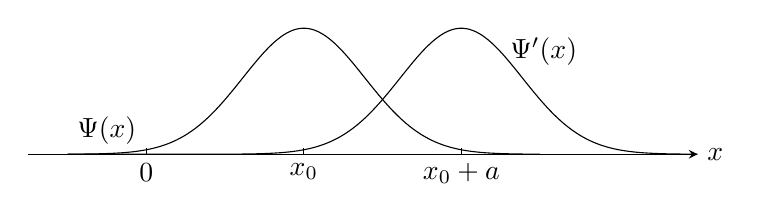
\begin{tikzpicture}[>=stealth]
        % assi
        \draw[->] (-0.5,0) -- (8,0) node[right] {$x$};
        % tacche e etichette
        \draw (1,0) -- (1,0.08) node[below,yshift=-2pt] {$0$};
        \draw (3,0) -- (3,0.08) node[below,yshift=-2pt] {$x_0$};
        \draw (5,0) -- (5,0.08) node[below,yshift=-2pt] {$x_0+a$};
        % profili d'onda (gaussiane stilizzate)
        \draw[smooth,domain=0:6,samples=200]
            plot(\x,{1.6*exp(-((\x-3)^2)/1.2)}) node[pos=0.28,above right] {$\Psi(x)$};
        \draw[smooth,domain=0:8,samples=200]
            plot(\x,{1.6*exp(-((\x-5)^2)/1.2)}) node[pos=0.78,above right , xshift = 5.5cm, yshift = 1cm] {$\Psi'(x)$};
    \end{tikzpicture}
    \caption{Traslazione di una funzione d'onda: $\Psi'(x)=\Psi(x-a)$.}
    \label{fig:traslazione-1d}
\end{figure}

L'operatore \(U(a)\) trasla la funzione d'onda, mentre l'operatore \(X'\) trasla il sistema di riferimento,
quindi i valori medi misurati sono gli stessi. 
Mentre l'operatore momento rimane invariato come ci si aspetta da una traslazione spaziale.

Per il teorema di Stone \ref{theo: Stone} deve esistere un generatore infinitesimo della trasformazione:
\[
    \bra{x} i\hbar\dv{a}U(a)\eval_{0}\ket{\Psi}= i\hbar \lim_{a\to 0 }   \frac{\bra{x}U(a)\ket{\Psi}-\braket{x}{\Psi}}{a}= i\hbar\lim_{a\to0 }\frac{\Psi(x-a)-\Psi(x)}{a} = -i\hbar \dv{x}\Psi(x)
\]
Che, in rappresentazione \(x\), corrisponde all'operatore momento \(P\) che dunque è il generatore infinitesimo di traslazioni:
\begin{equation}
    U(a) = e^{-\frac{i}{\hbar}aP}
\end{equation}


% Commutatore canonico e traslazioni generate da P
Supponiamo di partire da un sistema quantistico con
\[
    [Q,P]= i\hbar , \qquad Q,P \text{ a.a.}
\]
(coerente con la quantizzazione del corrispondente sistema classico).
Dato che \(P\) è a.a., l’operatore
\begin{equation}
    U(a)\equiv e^{-\frac{i}{\hbar}aP} \qquad a\in\mathbb{R}
\end{equation}
è un gruppo uniparametrico di operatori unitari.

\begin{equation}
    [Q,U(a)] =\left[ Q, e^{-\frac{i}{\hbar}aP} \right]     = aU(a)
\end{equation}


Sia \(\ket{q}\) un autovettore (generalizzato) di \(Q\): \(Q\ket{q}=q\ket{q}\): 
\[
    Q\,U(a)\ket{q}= \bigl(U(a)Q + aU(a)\bigr)\ket{q}
    = (q+a)\,U(a)\ket{q}
\]
Dunque \(U(a)\ket{q}\) è ancora autovettore di \(Q\) con autovalore \(q+a\).
Poiché \(a\in\mathbb{R}\) è arbitrario, segue che lo spettro di \(Q\) è traslato di qualsiasi quantità reale:
\[
    q\in\sigma(Q)\ \Longrightarrow\ q+a\in\sigma(Q)\ \ \forall\,a\in\mathbb{R}
    \quad\Longrightarrow\quad \sigma(Q)=\mathbb{R}
\]


Gli operatori \(U(a)=e^{-\frac{i}{\hbar}aP}\) realizzano le traslazioni di \(Q\);
equivalentemente, \(P\) è il generatore infinitesimo delle traslazioni della variabile coniugata a \(Q\).


\subsection{Traslazioni spaziali in 3D}

Sia \(\vec a=(a_x,a_y,a_z)\). Le traslazioni formano un gruppo abeliano a tre parametri:
\[
\tau(\vec a)\circ\tau(\vec b)=\tau(\vec a+\vec b)=\tau(\vec b)\circ \tau(\vec a)
\]
La rappresentazione unitaria \(U(\vec a)\) agisce su stati e osservabili come
\[
\ket{\Psi'}=U(\vec a)\ket{\Psi}, 
\qquad \Psi'(\vec x)=\Psi(\vec x-\vec a), 
\qquad U(\vec a)\,\vec X\,U(\vec a)^\dagger=\vec X-\vec a, 
\qquad U(\vec a)\,\vec P\,U(\vec a)^\dagger=\vec P .
\]

I generatori infinitesimi lungo gli assi sono \(P_x,P_y,P_z\) e, in generale,
\begin{equation}
    P_i \;=\; i\hbar\,\pdv{U(\vec a)}{a_i}\bigg|_{\vec a=0}\qquad i=x,y,z
\end{equation}
Per una traslazione nella direzione unitaria \(\hat n\):
\[
i\hbar\,\dv{s}U(s\hat n)\bigg|_{s=0}= \vec P\!\cdot\!\hat n
\]
e, dato un vettore arbitrario \(\vec a\),
\[
i\hbar\,\dv{s}U(s\vec a)\bigg|_{s=0}= \vec P\!\cdot\!\vec a
\]

Dal teorema di Stone segue dunque
\begin{equation}
    U(\vec a)=\exp\!\left(-\frac{i}{\hbar}\,\vec P\!\cdot\!\vec a\right)
\end{equation}
Poiché \([P_i,P_j]=0\) si può fattorizzare (l’ordine è irrilevante):
\[
U(\vec a)=e^{-\frac{i}{\hbar}P_x a_x}\,e^{-\frac{i}{\hbar}P_y a_y}\,e^{-\frac{i}{\hbar}P_z a_z}
\]

% 16 Lezione del 03/11/2025

\subsection{Rotazioni 3D}
\lezione{16}{03/11/2025}

Consideriamo la trasformazione di un vettore \(\vec{x} \in \mathbb{R}^3 \to \vec{x'}= R\vec{x}\), in cui consideriamo le matrici \(3\times3\) di rotazione \(R \) tali che \(R^\intercal R = I_3\) detto \textit{gruppo ortogonale} \(O(3)\).\\
Vale che \(\forall R \in O(3), \ \det R = \pm 1 \), tra queste consideriamo il \textit{gruppo speciale ortogonale}:
\begin{equation}
    SO(3)= \left\{ R \in O(3): \det R = +1 \right\}
\end{equation}
\(O(3)\) e \(SO(3)\) sono gruppi di Lie.

\begin{definition}
    \((G, \cdot )\) è \textit{gruppo di Lie} se \(G\) è varietà differenziabile e \(\cdot : G \times G \to G \) è differenziabile. 
\end{definition}

\begin{example}
    \(U(n)=\left\{ U \in \text{Mat}_{n\times n } : U^\dagger U = I \right\}\) detto \textit{gruppo unitario}.\\
    \(SU(n) = \left\{ U \in U(n ) : \det U = +1 \right\}\) detto \textit{gruppo unitario speciale}.
\end{example}


Consideriamo ora rotazioni infinitesime della forma \(R = I + s \delta R + O(s^2)\). Per la condizione \(R^\intercal R =I\) otteniamo:
\[
    I= (I+s \delta R^\intercal + \dots )(I+s \delta R+ \dots )= I + s(\delta R^\intercal+\delta R )
    \implies \delta R^\intercal=-\delta R 
\]
Cioè deve essere una matrice antisimmetrica. Una base per lo spazio delle matrici antisimmetriche, detto \textit{algebra di Lie} di \(SO(3)\) e indicata con \(so(3)\), è data da:
\[
    T_1=\begin{pmatrix}
        0 & 0 & 0\\
        0 & 0 & -1\\
        0 & 1 & 0
    \end{pmatrix},\qquad
    T_2=\begin{pmatrix}
        0 & 0 & 1\\
        0 & 0 & 0\\
        -1 & 0 & 0
    \end{pmatrix},\qquad
    T_3=\begin{pmatrix}
        0 & -1 & 0\\
        1 & 0 & 0\\
        0 & 0 & 0
    \end{pmatrix} .
\]
I loro elementi sono compattiamente scritti come
\[
    (T_k)_{ij} = -\,\epsilon_{kij} \qquad i,j,k=1,2,3
\]
con $\epsilon_{kij}$ simbolo di Levi\,–\,Civita. \\
Se definiamo 
\[
    \vec T=(T_1,T_2,T_3)\,, \quad \vec\omega=(\omega_1,\omega_2,\omega_3)
\]
abbiamo che 
ogni matrice \(R \in SO(3)\) è data da \(R = e^{\vec{\omega}\cdot \vec{T}}\equiv R(\omega)\) e indica la rotazione lungo l'asse \(\vec{\omega}\) di un angolo \(\abs{\vec{\omega}}\).


\begin{example}
    \[
        \vec{\omega}= \begin{pmatrix}
            0\\0\\\pi/3
        \end{pmatrix}\implies e^{\frac{\pi}{3}T_3} = \begin{pmatrix}
            \cos \frac{\pi}{3}& - \sin \frac{\pi}{3} & 0\\
            \sin \frac{\pi}{3} &\cos \frac{\pi}{3} & 0\\
            0&0&1
        \end{pmatrix}
    \]
\end{example}
\begin{remark}
    Vale la relazione: \(T_k = \pdv{R(\vec{\omega})}{\omega_k}\eval_{\vec{\omega}=0}\).
\end{remark}

\begin{remark}
    In genereale, \(e^{\vec{\omega}\cdot\vec{T}}e^{\vec{\omega'}\cdot\vec{T}} \neq e^{(\vec{\omega}+\vec{\omega'})\cdot\vec{T}}\) perché \(\left[ T_i, T_j \right]= \sum_k \epsilon_{ijk}T_k \neq 0\) .
\end{remark}

Vediamo ora sistemi quantistici con simmetria \(SO(3)\). A ogni \(R(\vec{\omega}) \in SO(3)\) per il teorema di Wigner \ref{theo: Wigner} deve essere associato un operatore unitario \(U_{R(\vec{\omega})}\equiv U(\vec{\omega})= e^{-\frac{i}{\hbar}\vec{\omega}\cdot\vec{J}}\).\\
Nella stessa maniera in cui \(SO(3)\) induce un algebra di Lie \(so(3)\), \(U_{R(\vec{\omega})}\) induce per il teorema di Stone \ref{theo: Stone} un insieme di operatori a.a.:
\begin{equation}
    \frac{1}{i\hbar} J_k := \pdv{U(\vec{\omega})}{\omega_k}\eval_{\vec{\omega}=0}
\end{equation}

Dunque se \(U(\vec{\omega})\) è rappresentazione unitaria non proiettiva di \(SO(3)\) e \(\frac{1}{i\hbar}J_k\) sono rappresentazione autoaggiunta di \(so(3)\) e dovranno avere le stesse relazioni di commutazione:
\begin{equation}
    \left[ J_i , J_k\right] = i\hbar\sum_k \epsilon_{ijk} J_k
\end{equation}
I \(J_k\) corrispondono alle componenti del momento angolare.

Se invece \(U(\vec{\omega})\) è rappresentazione genuinamente proiettiva, ottengo:
\[
    \left[ J_i , J_k\right] = i\hbar\sum_k \epsilon_{ijk} J_k + c_{ij} I 
\]
ma nel caso di \(so(3)\) si può sempre porre \(c_{ij}= 0 \ \forall\,i,j\) .\\
Inoltre, si ha il problema che per \(\vec{\omega}= (0 \ 0 \ \pi)\) avrò:
\[
    R(\vec{\omega })R(\vec{\omega}) = I  \quad  \text{ ma }\quad  U_{R(\vec{\omega}) }U_{R(\vec{\omega}) }= \pm I 
\]


\begin{example}
    \textbf{Particella in 3D senza spin}
    \[
        \mathcal{H} = L_2(\mathbb{R}) \quad R \in SO(3)\qquad
        \ket{\Psi' }= U(R)\ket{\Psi} \qquad \Psi'(\vec{x})= \Psi(R^{-1}\vec{x}) 
    \]
    \[
        U(R)\vec{X}U(R)^\dagger = R^{-1} \vec{X}    \qquad U(R)\vec{P}U(R)^\dagger = R^{-1}\vec{P}  
    \]
    Il generatore infinitesimo è dato da \(J_k = i\hbar  \pdv{U(\vec{\omega})}{\omega_k}\eval_{\vec{\omega}=0}\) 
    e vogliamo mostrare che in questo sistema: \(\vec{J}= \vec{L}:= \vec{X}\times \vec{P}\) con \( L_k = \sum_{i,j}\epsilon_{kij}X_i P_j\)

    \[
    \bra{\vec{x}}J_k\ket{\Psi}
    = i\hbar\,\pdv{}{\omega_k}\bra{\vec{x}}U(\vec{\omega})\ket{\Psi}\eval_{\vec{\omega}=0}
    = i\hbar\,\pdv{}{\omega_k}\Psi\!\big(R(\vec{\omega})^{-1}\vec{x}\big)\eval_{\vec{\omega}=0}
    \]

    \[
    = i\hbar\sum_{j=1}^{3}(\pdv{x_j}\Psi)\,\pdv{}{\omega_k}\!\left[(R(-\vec{\omega})\vec{x})_j\right]\eval_{\vec{\omega}=0}
    \]

    Sviluppando \(R(-\vec{\omega})=I-\sum_m\omega_mT_m+\dots\) con 
    \((T_m)_{j\ell}=-\epsilon_{m j \ell}\), si ha:
    \[
    (R(-\vec{\omega})\vec{x})_j = x_j - \sum_{k,\ell}\omega_k(T_k)_{j\ell}x_\ell+ \dots
    = x_j - \sum_{k,\ell}\omega_k\epsilon_{k \ell j}x_\ell + \dots
    \]

    \[
    \implies \pdv{}{\omega_k} \left(R(-\vec{\omega})\vec{x}\right)_j\eval_{\vec{\omega}=0}
    = \sum_{\ell}-\epsilon_{k  \ell j}x_\ell
    \]

    \[
    \implies \bra{\vec{x}}J_k\ket{\Psi}
    = i\hbar\sum_{j,\ell}-\epsilon_{k  \ell j}x_\ell(\pdv{j}\Psi)
    = \sum_{j,\ell}\epsilon_{k\ell j}x_\ell(-i\hbar\pdv{j})\Psi
    = \sum_{j,\ell}\epsilon_{k\ell j}X_\ell P_j\Psi
    \]

    \[
    \boxed{J_k = \sum_{j,\ell}\epsilon_{k\ell j}X_\ell P_j = L_k}
    \]
    Vale inoltre: \(\left[ L_i, L_j \right]= i\hbar \sum_k \epsilon_{ijk} L_k\)

    \begin{attention}
        \(\vec{L}\) è il momento angolare orbitale, \(\vec{J}\) è il momento angolare totale. In alcuni sistemi fisici \(\vec{J}\neq \vec{L}\).
    \end{attention}
\end{example}

\begin{definition}
    Se ho terna di operatori \(\vec{V}\equiv (V_1,V_2,V_3)\), si dice che la terna trasforma come un vettore per \(SO(3)\) se e solo se:
    \begin{equation}
        \left[ J_j, V_k  \right]= i\hbar \sum_{l}\epsilon_{jkl}V_l \iff U(\vec{\omega}) V_j U (\vec{\omega})^\dagger = \sum_{k} R(\vec{\omega})^{-1}_{jk}V_k
    \end{equation}
\end{definition}
\begin{definition}
    Diciamo che un operatore \(S\) è \textit{scalare} per rotazioni se vale:
    \begin{equation}
        \left[ J_i,S \right]=0 \quad i = 1,2,3 \qquad \ U(\vec{\omega})S U(\vec{\omega})^{\dagger} = S
    \end{equation}
\end{definition}
\begin{example}
    Se ho una terna che traforma come vettore ad esempio \(\vec{P}\), i loro moduli ad esempio \(P^2 = \vec{P}\cdot \vec{P}\) sono scalari.
\end{example}


% 17 Lezione del 04/10/2025

\subsubsection{Rototraslazioni}
\lezione{17}{04/10/2025}

Una rototraslazione è una trasformazione descritta da:
\begin{equation}
    g = (R, \vec{a})= (I, \vec{a})(R,0) \qquad \vec{x}'= (R, \vec{a})\vec{x}= R\vec{x}+ \vec{a}
\end{equation}
definita in modo che prima avvenga la rotazione e successivamente la traslazione.\\
Le rototraslazioni formano ovviamente un gruppo, la cui identità: \(id = (I,0)\), l'inversa è \((R,\vec{a})^{-1}= (R^{-1}, -R^{-1}\vec{a})\) e la composizione vale:
\[
(R_1,\vec{a_1})(R_2, \vec{a_2})\vec{x}= (R _1, \vec{a})(R_2\vec{x}+\vec{a_2})= R_1R_2\vec{x}+ R_1\vec{a}+ \vec{a_1}= (R_1R_2, R_1\vec{a_2}+\vec{a_1})
\]
Che verifica la definizione di inversa:
\[
    (R, \vec{a})(R^{-1}, R^{-1}\vec{a}) = (I, - RR^{-1}\vec{a}+\vec{a})= (I,0)
\]
Essendo una composizione di rotazioni e traslazioni la rappresentazione unitaria è data da:
\[
    U_{(R, \vec{a})}= U_{\vec{a}}U_{R(\vec{\omega})}= e^{-\frac{i}{\hbar}\vec{P}\cdot\vec{a}}e^{-\frac{i}{\hbar}\vec{\omega}\cdot\vec{j}}
\]
Abbiamo quindi un gruppo a 6 parametri generato da le \(J_i e P_i\), la cui algebra è data da:
\[
    \left[ J_i, J_j  \right]= i\hbar \sum_k\epsilon_{ijk}J_k \qquad 
    \left[ P_i, P_j \right] =0 \qquad \left[ J_i, P_j\right] = i\hbar \sum_k    \epsilon_{ijk}P_k
\]




\section{Simmetrie della dinamica}
Consideriamo \(\ket{\Psi(t)}\) soluzione equazione di Schrödinger e una simmetria \(\tau\) descritta da un operatore unitario e indipendente dal tempo \(W\).\\
\(\ket{\Psi'(t)}= W\ket{\Psi(t)} \ \forall\,t \) è ancora soluzione dell'eq di Schrödinger? 
\[
    i\hbar\dv{t}W\ket{\Psi(t)} =   W i\hbar \dv{t}\ket{\Psi(t)} = W H(t)\ket{\Psi(t)} \equiv H(t)W\ket{\Psi(t)}  \iff \left[ W, H(t) \right]=0
\]

\begin{definition}
    Definiamo il \textit{gruppo di simmetrie della dinamica} come:
    \begin{equation}
        G_d = \left\{ W \text{ (anti)unitari }  : \ \left[ W, H \right]=0 \right\} \subseteq G
    \end{equation}
    Questo è equivalente a \(WHW^\dagger= H\) e se \(W\) è unitario (non anti) allora \(\left[ W, U(t,t_0) \right]=0\)
\end{definition}

Nella visuale di Heisenberg, con \(A_h(t)= U(t-t_0)^\dagger A_s U(t-t_0)\)
se \(W \in G_d\) vale:
\[
    WA_h(t)W^\dagger = U(t-t_0)^\dagger W A_s W^\dagger U(t-t_0)
\]
è ancora soluzione dell'eq di Heisenberg.

Se \(W\) formano un gruppo a un parametro \(W(s)= e^{-\frac{i}{\hbar}sQ}\) vale:
\begin{equation}
    \left[ W(s), H \right]= 0 \ \forall\, s \iff \left[ Q, H \right]    =0 \iff \dv{t} \expval{Q}_\Psi (t)=0 \quad \forall\, \Psi \in \mathcal{H}
\end{equation}
Esiste relazione diretta tra simmetrie di un sistema e quantità conservate.

\begin{theorem}\label{theo: Noether}
    {\normalfont\textbf{di Noether in MQ}}\\
    \(H\) è invariante per simmetria generata da operatore \(Q\) autoaggiunto se e solo se \(Q\) è quantità conservata.
\end{theorem}

\begin{remark}
    Dato \(W\) unitario, \(\left[ W, H \right]=0\) e \(H\ket{E}= E\ket{E}\), allora:
    \begin{equation}
        HW\ket{E} = WH\ket{E}= EW\ket{E}
    \end{equation}
    \(W\ket{E}\) è ancora autovettore di \(H\) con stesso autovalore.
\end{remark}

\begin{remark}
    Se esistono due autovettori \(\ket{E,1}\) e \(\ket{E,2}\) degeneri di \(H\), tali che \(\braket{E,r}{E,s}= \delta_{rs}\),
    allora esite operatore unitario \(W\) tale che:
    \begin{equation}
        \left[ W, H \right]= 0 \quad \begin{cases}
                W\ket{E,1}= \ket{E,2}\\ W\ket{E,2}=\ket{E,1}
            \end{cases}
    \end{equation}
\end{remark}
\begin{proof}
    Data \(\left\{ \ket{E,1}\equiv \ket{1}, \ket{E,2}\equiv \ket{2}, \ket{3},\ket{4}, \dots  \right\}\) base ON di autovettori di \(H\), definisco mappa lineare \(W\) tale che:
    \[
        W\ket{E,1}= \ket{E,2} \quad  W\ket{E,2}=\ket{E,1} \qquad W\ket{n}= \ket{n} \quad n\geq 3
    \]
    è unitario perché mappa base ON in base ON e vale \((WH-HW)\ket{n}=0 \quad \forall,n\)
\end{proof}

Di consueguenza sappiamo che se \(\sigma(H)\) è completamente non degenere \(\left\{ \ket{E} \right\}_{E \in \sigma(H)}\) e \(W \) unitario \(\left[ W, H \right]=0\), 
allora per la prima osservazione abbiamo che \(W\ket{E}= f(E)\ket{E}\) con \(f(E)\in \mathbb{C} \quad \forall, E \in \sigma(H)\), dunque \(W = f(H)\). 
Chiamiamo tali operatori \textit{gruppo di simmetrie banali della dinamica}:
\begin{equation}
    K_d:= \left\{ W \text{ unitari } : \ W = f(H) \right\}   \subseteq G_d
\end{equation}
Perciò se \(\sigma(H)\) è completamente non degenere, \(K_d= G_d\)  e tutte le simmetrie delle dinamica possibili sono banali.\\
Se invece \(E \in \sigma(H)\) è degenere, per la seconda osservazione esiste un \(W \in G_d, \ W \notin K_d\), cioè ammette simmetrie non banali.


\subsection{Traslazioni temporali}
L'omogeneità nel tempo per sistemi conservativi induce una simmetria per traslazioni temporali, data da un gruppo ad un parametro \(U(t)= e^{-\frac{i}{\hbar}Ht}\) che trasforma:
\[
    \ket{\Psi'}= U(t)\ket{\Psi} \qquad A'=U(t)AU(t)^\dagger 
\]
\begin{attention}
    Non si tratta di evoluzione causale, stiamo cambiando sia le funzione d'onda che gli operatori e le medie rimangono invariate. 
    Invece, nell'evoluzione casuale, cambiano solo le funzioni d'onda nella visuale di Schrödinger o solo gli operatori in quella di Heisenberg.
\end{attention}


\section{Simmetrie discrete}
\subsection{Parità Spaziale}
Consideriamo ora la riflessione rispetto all'origine: \(\vec{x}\to -\vec{x}\) descritta dalla matrice:
\[
    R_p = \begin{pmatrix}
        -1&0&0\\0&-1&0\\0&0&-1
    \end{pmatrix}
    \in O(3) \quad \notin SO(3) \ (\det = -1)
\]
Notiamo che tutte le \textit{rotazioni impoprie} cioè \(\forall\, g \in O(3) \ \notin SO(3)\) possono essere scritte come \(g = R_pR(\vec{\omega})\) con \(R(\vec{\omega})\in SO(3)\).

Consideriamo una particella senza spin in 3D e un operatore \(\mathbb{P}\) che agisce come:
\[
    \mathbb{P}\vec{X}\mathbb{P}^\dagger = -\vec{X} \qquad \mathbb{P}\vec{P}\mathbb{P}^\dagger = -\vec{P} \qquad \mathbb{P}\vec{L}\mathbb{P}^\dagger = \vec{L}  
\]
Gli operatori \(\vec{X}\) e \(\vec{P}\) per questo si dicono \textit{vettori polari} e \(\vec{L}\) si dice \textit{vettore assiale}.


Verifichiamo se \(\mathbb{P}\) è unitario o antiunitario:
\begin{equation*}
\left[ \, \mathbb{P} X_j \mathbb{P}^\dagger ,\, \mathbb{P} P_k \mathbb{P}^\dagger \right]
= \mathbb{P}\,[X_j,P_k] \,\mathbb{P}^\dagger
= \mathbb{P}\,(i\hbar\,\delta_{jk})\,\mathbb{P}^\dagger 
= \begin{cases}
 i\hbar\,\delta_{jk}, & \mathbb{P} \text{ unitario},\\
 -i\hbar\,\delta_{jk}, & \mathbb{P} \text{ antiunitario}.
 \end{cases}
\end{equation*}

Dalla definizione di \(\mathbb{P}\) otteniamo:
\[
\left[ \, \mathbb{P} X_j \mathbb{P}^\dagger ,\, \mathbb{P} P_k \mathbb{P}^\dagger \right]
= [-X_j,-P_k] = i\hbar\,\delta_{jk}.
\]
Confrontando i due risultati segue che \(\mathbb{P}\) è unitario.

Dato che \(\mathbb{P}^2 = I\) segue che \(\mathbb{P}= \mathbb{P}^{-1}= \mathbb{P}^\dagger\) cioé è sia unitario che autoaggiunto.\\
Lo spettro \(\sigma(\mathbb{P})= \left\{ \pm 1   \right\}\), dunque per autovalore \(n_p \in \sigma(\mathbb{P})\) vale:
\[
    \bra{\vec{x}}\mathbb{P}\ket{\Psi}= n_p\braket{\vec{x}}{\Psi} \iff \Psi(-\vec{x}) = n_p \Psi(\vec{x})
\]
dunque gli autostati di \(n_p=1\) sono le funzioni d'onda pari, per \(n_p= -1\) le funzioni d'onda dispari.

Per l'operatore hamiltoniano:
\[
    H = \frac{\abs{\vec{P}}^2}{2m} + V(\vec{x}) \to \mathbb{P}H\mathbb{P}= \frac{\abs{\vec{P}}^2}{2m} + V(-\vec{x}) 
\]
Perciò se \(V(\vec{x})= V(-\vec{x})\) allora \(\mathbb{P} \in G_d\).



% 18 Lezione del 07/11/2025

\subsection{Inversione temporale}
\lezione{18}{07/11/2025}

Consideriamo l'operatore \(\mathbb{T}\) che agisca nella seguente maniera:
\[
    \vec{x}\to \vec{x} \quad t \to -t \qquad \mathbb{T}\vec{X}\mathbb{T}^\dagger = \vec{X} \qquad  \mathbb{T}\vec{P}\mathbb{T}^\dagger = - \vec{P} \qquad  \mathbb{T}\vec{L}\mathbb{T}^\dagger = - \vec{L}
\]

In questo caso:
\begin{align*}
    \left[ \mathbb{T}X_j\mathbb{T}^\dagger,\mathbb{T}P_k\mathbb{T}^\dagger \right] 
    &= \mathbb{T}\left[ X_j, P_k \right]\mathbb{T}^\dagger = \mathbb{T}i \hbar \delta_{jk}\mathbb{T}^\dagger \\
    &= - \left[ X_j, P_k \right] = -i\hbar \delta_{jk}
\end{align*}
Dunque \(\mathbb{T}\) è antiunitario, perciò \(\braket{\chi}{\mathbb{T}\Psi}= \overline{\braket{\mathbb{T}\chi}{\Psi}}\).
Come agisce \(\mathbb{T}\) sullo stato \(\ket{\Psi}\) ?
\[
    \mathbb{T}\ket{\Psi}= \mathbb{T}\int_{\mathbb{R}^3}\dd[3]{x}\ket{\vec{x}}\braket{\vec{x}}{\Psi} = \int_{\mathbb{R}^3}\dd[3]{x}\ket{\vec{x}}\braket{\vec{x}}{\Psi}^*
    \implies \Psi'(\vec{x})= \Psi(\vec{x})^*
\]
Un sistema è invariante per inversione temporale se l'Hamiltoniana \(H\) commuta con \(\mathbb{T}\).
\[
    [\mathbb{T}, H] = 0 \iff H = \mathbb{T} H \mathbb{T}^\dagger
\]
Per un sistema conservativo, l'operatore di evoluzione temporale \(U(t) = e^{-\frac{i}{\hbar}Ht}\) si trasforma come:
\begin{equation}
    \mathbb{T} U(t) \mathbb{T}^\dagger = \mathbb{T} e^{-\frac{i}{\hbar}Ht} \mathbb{T}^\dagger = e^{\frac{i}{\hbar}Ht} = U(-t)
\end{equation}
Data una soluzione dell'equazione di Schrödinger \(\ket{\Psi(t)} = U(t)\ket{\Psi(0)}\), lo stato trasformato \(\mathbb{T}\ket{\Psi(t)}\) evolve come:
\[
    \mathbb{T}\ket{\Psi(t)} = \mathbb{T} U(t) \mathbb{T}^\dagger \mathbb{T}\ket{\Psi(0)} = U(-t) \mathbb{T}\ket{\Psi(0)}
\]
Questo stato \textbf{non è una soluzione} dell'equazione di Schrödinger, poiché la sua evoluzione temporale è invertita rispetto a quella richiesta.

Tuttavia, se definiamo un nuovo stato \(\ket{\Psi'(t)}\) come lo stato originale evoluto all'indietro nel tempo e poi trasformato con \(\mathbb{T}\):
\[
    \ket{\Psi'(t)} := \mathbb{T}\ket{\Psi(-t)}
\]
allora \(\ket{\Psi'(t)}\) \textbf{è una soluzione} dell'equazione di Schrödinger.
Infatti:
\[
    \ket{\Psi'(t)} = \mathbb{T} U(-t) \ket{\Psi(0)} = \left( \mathbb{T} U(-t) \mathbb{T}^\dagger \right) \mathbb{T}\ket{\Psi(0)} = U(t) \mathbb{T}\ket{\Psi(0)}
\]
Lo stato \(\ket{\Psi'(t)}\) evolve correttamente a partire da un nuovo stato iniziale \(\ket{\Psi'(0)} = \mathbb{T}\ket{\Psi(0)}\).

Nella rappresentazione delle coordinate, questo significa che se \(\Psi(\vec{x}, t)\) è una soluzione, allora lo è anche la sua complessa coniugata con il tempo invertito.
\[
    \braket{\vec{x}}{\Psi'(t)} = \braket{\vec{x}}{\mathbb{T} | \Psi(-t)} = \braket{\vec{x}}{\Psi(-t)}^* = \Psi^*(\vec{x}, -t)
\]

Se \(\Psi(\vec{x}, t)\) è soluzione all'equazione di Schrödinger per un sistema con simmetria di inversione temporale, allora lo è anche \(\Psi^*(\vec{x}, -t)\).



\subsection{Spettro del momento angolare}
Consideriamo un sistema quantistico con simmetria di rotazione \(SO(3)\).
Il momento angolare totale \(\vec{J} = (J_x, J_y, J_z)\) è un insieme di operatori autoaggiunti che generano le rotazioni tramite \(U(\vec{\alpha}) = e^{-\frac{i}{\hbar}\vec{\alpha} \cdot \vec{J}}\)
e obbediscono all'algebra di Lie di \(so(3)\):
\begin{equation}
    [J_i, J_j] = i\hbar \sum_k \epsilon_{ijk} J_k
\end{equation}
Per studiare lo spettro, ci concentriamo su \(J_z\), ma i risultati si estendono a \(J_x\) e \(J_y\) per simmetria.
\begin{remark}
    Gli spettri delle componenti del momento angolare coincidono, \(\sigma(J_z) = \sigma(J_x) = \sigma(J_y)\),
    poiché le componenti sono collegate da trasformazioni unitarie (rotazioni).
\end{remark}

Definiamo l'operatore \(\vec{J}^2 = J_x^2 + J_y^2 + J_z^2\), che è uno scalare rotazionale e quindi commuta con tutte le componenti di \(\vec{J}\):
\[
    [\vec{J}^2, J_k] = 0
\]
Per trovare lo spettro di \(J_z\), introduciamo gli \textit{operatori di innalzamento e abbassamento} (o operatori scala):
\begin{equation}
    J_\pm := J_x \pm i J_y.
\end{equation}
Valgono le seguenti proprietà:
\[
    (J_\pm)^\dagger = J_\mp, \qquad \left[ \vec{J}^2, J_\pm \right] = 0, \qquad J_x = \frac{J_+ + J_-}{2}, \qquad J_y = \frac{J_+ - J_-}{2i}.
\]
Inoltre, valgono le relazioni di commutazione:
\[
    [J_z, J_\pm] = [J_z, J_x] \pm i[J_z, J_y]
    = (i\hbar J_y) \pm i(-i\hbar J_x) = \pm \hbar (J_x \pm i J_y) = \pm \hbar J_\pm.
\]
I prodotti \(J_+ J_-\) e \(J_- J_+\) si possono esprimere in termini di \(\vec{J}^2\) e \(J_z\):
\[
    J_+ J_- = (J_x + i J_y)(J_x - i J_y) = J_x^2 + J_y^2 - i[J_x, J_y] = J_x^2 + J_y^2 + \hbar J_z = \vec{J}^2 - J_z^2 + \hbar J_z,
\]
\[
    J_- J_+ = (J_x - i J_y)(J_x + i J_y) = J_x^2 + J_y^2 + i[J_x, J_y] = J_x^2 + J_y^2 - \hbar J_z = \vec{J}^2 - J_z^2 - \hbar J_z.
\]
Da cui si ricava il commutatore:
\[
    [J_+, J_-] = 2\hbar J_z.
\]

L'operatore \(\vec{J}^2\) è semidefinito positivo. Infatti, per ogni stato \(\ket{\Psi}\):
\[
    \expval{\vec{J}^2}_\Psi = \bra{\Psi} (J_x^2 + J_y^2 + J_z^2) \ket{\Psi}
    = \norm{J_x \ket{\Psi}}^2 + \norm{J_y \ket{\Psi}}^2 + \norm{J_z \ket{\Psi}}^2 \ge 0.
\]
Di conseguenza, il suo spettro è non negativo: \(\sigma(\vec{J}^2) \subseteq \mathbb{R}_{\ge 0}\).

Poiché \([\vec{J}^2, J_z]=0\), possiamo trovare una base ortonormale di autostati comuni \(\left\{ \ket{j, m} \right\}\).
Definiamo i loro autovalori:
\begin{align}
    \vec{J}^2 \ket{j, m} &= \hbar^2 j(j+1) \ket{j, m}, \quad j \ge 0 \\
    J_z \ket{j, m} &= \hbar m \ket{j, m}, \quad m \in \mathbb{R}
\end{align}
La parametrizzazione dell'autovalore di \(\vec{J}^2\) come \(\hbar^2 j(j+1)\) è una scelta standard che si rivelerà conveniente. La condizione \(\vec{J}^2 \ge 0\) è soddisfatta per \(j \ge 0\).

Applichiamo ora gli operatori scala \(J_\pm\) agli autostati \(\ket{j,m}\). Poiché \([\vec{J}^2, J_\pm]=0\), il valore di \(j\) non cambia:
\[
    \vec{J}^2 (J_\pm \ket{j, m}) = J_\pm \vec{J}^2 \ket{j, m} = \hbar^2 j(j+1) (J_\pm \ket{j, m}).
\]
Invece, l'autovalore di \(J_z\) viene traslato:
\[
    J_z (J_\pm \ket{j, m}) = (J_\pm J_z + [J_z, J_\pm]) \ket{j, m}
    = (J_\pm \hbar m \pm \hbar J_\pm) \ket{j, m}
    = \hbar (m \pm 1) (J_\pm \ket{j, m}).
\]
Lo stato \(J_\pm \ket{j, m}\) è quindi un autostato di \(J_z\) con autovalore \(\hbar(m\pm 1)\).

Perché \(J_\pm \ket{j, m}\) sia un autostato valido, non deve essere il vettore nullo. Calcoliamone la norma (assumendo \(\braket{j, m}{j, m} = 1\)):
\[
    \norm{J_\pm \ket{j, m}}^2 = \bra{j, m} J_\mp J_\pm \ket{j, m}
    = \bra{j, m} (\vec{J}^2 - J_z^2 \mp \hbar J_z) \ket{j, m}
\]
Sostituendo gli autovalori, otteniamo:
\[
    \norm{J_\pm \ket{j, m}}^2 = \hbar^2 [j(j+1) - m^2 \mp m]
    = \hbar^2 [j(j+1) - m(m \pm 1)]
\]
Poiché la norma quadra deve essere non negativa, abbiamo due condizioni:
\begin{align*}
    \norm{J_+ \ket{j,m}}^2 \ge 0 \implies j(j+1) - m(m+1) \ge 0 \\
    \norm{J_- \ket{j,m}}^2 \ge 0 \implies j(j+1) - m(m-1) \ge 0
\end{align*}
Queste due disequazioni sono entrambe soddisfatte se e solo se:
\begin{equation}
    -j \le m \le j.
\end{equation}
Per un dato \(j\), i valori di \(m\) sono quindi limitati.

La sequenza di autostati \(\dots, \ket{j, m-1}, \ket{j, m}, \ket{j, m+1}, \dots\) deve essere finita.
Ciò accade quando il vettore diventa nullo:
\begin{itemize}
    \item Deve esistere un \(m_\text{max}\) tale che \(J_+ \ket{j, m_\text{max}} = 0\).
    Dalla condizione sulla norma, \(j(j+1) - m_\text{max}(m_\text{max}+1) = 0\), che implica \(m_\text{max} = j\).
    \item Deve esistere un \(m_\text{min}\) tale che \(J_- \ket{j, m_\text{min}} = 0\).
    Similmente, \(j(j+1) - m_\text{min}(m_\text{min}-1) = 0\), che implica \(m_\text{min} = -j\).
\end{itemize}
Partendo da \(m_\text{min} = -j\), si deve poter raggiungere \(m_\text{max} = j\) con un numero intero \(k\) di passi da \(+1\) (applicando \(J_+\) ripetutamente):
\[
    m_\text{max} - m_\text{min} = k, \quad k \in \mathbb{Z}_{\ge 0}
\]
\[
    j - (-j) = k \implies 2j = k.
\]
Questo implica che \(2j\) deve essere un numero intero non negativo. I valori possibili per \(j\) sono quindi:
\[
    j = 0, \frac{1}{2}, 1, \frac{3}{2}, \dots
\]
Per un dato \(j\), i valori permessi di \(m\) sono \(2j+1\) valori equispaziati:
\[
    m = -j, -j+1, \dots, j-1, j.
\]




% 19 Lezione del 10/11/2025
\lezione{19}{10/11/2025}
Consideriamo una base ON di autostati \(\left\{ \ket{j,m} \right\} \)  per un certo \( j\) fissato con \(m \in \{-j, \dots, j\}\).

Partendo dall'autostato dell'autovalore più grande \(m=j\,, \ \  \norm{\ket{j,j}}^2 = 1\), posso ottenere gli altri elementi della base grazie all'operatore di abbassamento:
\[
    \ket{j, m-1} := \frac{J_- \ket{j,m}}{\hbar \sqrt{j(j+1) - m(m-1)}} \quad \text{per } m > -j
\]
Che viene opportunamente normalizzato. Alla stessa maniera l'operatore di innalzamento agisce come:
\[
    J_+ \ket{j,m} = \frac{J_+ J_- \ket{j,m+1}}{\hbar \sqrt{j(j+1) - m(m+1)}} = \hbar \sqrt{j(j+1)-(m+1)m} \ket{j, m+1}
\]

Quindi gli operatori di innalzamento e abbassamento, aumentano e diminuiscono rispettivamente l'autovalore \(m \) e aggiungono un fattore di proporzione dipendente da \(j\) e \(m\):
\begin{equation}
    J_\pm \ket{j,m} = \hbar \sqrt{j(j+1)-m(m\pm 1)} \ket{j, m \pm 1}
\end{equation}

Rispetto a questa base ortonormale \(\left\{ \ket{j,m} \right\}_{m=-j}^j\) (con \(j\) fissato), le rappresentazioni matriciali degli operatori del momento angolare hanno una forma conveniente:
\begin{itemize}
    \item Per \(J_z\), la rappresentazione è diagonale:
    \[
        \matrixel{j,m'}{J_z}{j,m} = m\hbar\,\delta_{m'm}
        \implies
        J_z = \hbar \begin{pmatrix} j & & & 0 \\ & j-1 & & \\ & & \ddots & \\ 0 & & & -j \end{pmatrix}.
    \]
    \item Per gli operatori scala \(J_\pm\), definendo per brevità $\mu_\pm(j,m) = \hbar \sqrt{j(j+1)-m(m\pm 1)}$, si ha:
    \[
        \matrixel{j,m'}{J_+}{j,m} = \mu_+(j,m)\,\delta_{m',m+1},
        \qquad
        \matrixel{j,m'}{J_-}{j,m} = \mu_-(j,m)\,\delta_{m',m-1}.
    \]
    Le matrici corrispondenti sono strettamente triangolari, con elementi non nulli solo sulla prima sovradiagonale per \(J_+\) e sulla prima sottodiagonale per \(J_-\).
    \[
        J_+ = \begin{pmatrix} 0 & \mu_+(j,j-1) & 0 & \dots \\ 0 & 0 & \mu_+(j,j-2) & \dots \\ \vdots & & \ddots & \mu_+(j,-j) \\ 0 & \dots & \dots & 0 \end{pmatrix},
    \]
    \[
        J_- = \begin{pmatrix} 0 & 0 & \dots & 0 \\ \mu_-(j,j) & 0 & \dots & 0 \\ 0 & \mu_-(j,j-1) & \ddots & \vdots \\ \vdots & & \ddots & 0 \\ 0 & \dots & \mu_-(j,-j+1) & 0 \end{pmatrix}.
    \]
    \item Per \(J_x\) e \(J_y\), le matrici si ottengono dalle relazioni \(J_x = (J_+ + J_-)/2\) e \(J_y = (J_+ - J_-)/(2i)\).
    Sono matrici tridiagonali con elementi nulli sulla diagonale principale.
    \[
        J_x = \frac{1}{2} \begin{pmatrix} 0 & \mu_+(j,j-1) & & 0 \\ \mu_-(j,j) & 0 & \mu_+(j,j-2) & \\ & \mu_-(j,j-1) & \ddots & \mu_+(j,-j) \\ 0 & & \mu_-(j,-j+1) & 0 \end{pmatrix},
    \]
    \[
        J_y = \frac{1}{2i} \begin{pmatrix} 0 & \mu_+(j,j-1) & & 0 \\ -\mu_-(j,j) & 0 & \mu_+(j,j-2) & \\ & -\mu_-(j,j-1) & \ddots & \mu_+(j,-j) \\ 0 & & -\mu_-(j,-j+1) & 0 \end{pmatrix}.
    \]
\end{itemize}


\subsubsection{Spettro degenere}

Se è presente degenerazione, l'autospazio \(\mathcal{H}_{j,m}\) associato agli autovalori \(j(j+1)\hbar^2\) e \(m\hbar\) ha dimensione \(d(j,m) > 1\).
Si considera una base ortonormale di questo autospazio, indicizzata da un numero quantico aggiuntivo $r$:
\[
    \{ \ket{j, m, r} \}_{r=1, \dots, d(j,m)}
\]
tale che $\braket{j, m, r}{j, m, r'} = \delta_{rr'}$.

Analizziamo l'azione degli operatori di scala, che agiscono sull'indice $m$ ma non sull'indice di degenerazione $r$.
Per \(m > -j\), l'operatore di abbassamento \(J_-\) mappa lo stato \(\ket{j, m, r}\) in un nuovo stato. Definiamo i vettori normalizzati:
\[
    \ket{j, m-1, r} := \frac{J_- \ket{j, m, r}}{\hbar \sqrt{j(j+1) - m(m-1)}}
\]
Questi vettori sono ortonormali rispetto all'indice $r$:
\[
    \braket{j, m-1, r}{j, m-1, r'} = \delta_{rr'}
\]
Poiché abbiamo costruito un sistema ortonormale di \(d(j,m)\) vettori nell'autospazio \(\mathcal{H}_{j, m-1}\), la sua dimensione deve essere almeno \(d(j,m)\):
\[
    d(j, m-1) \ge d(j, m)
\]

Allo stesso modo, per \(m < j\), l'operatore di innalzamento \(J_+\) permette di definire i vettori normalizzati:
\[
    \ket{j, m+1, r} := \frac{J_+ \ket{j, m, r}}{\hbar \sqrt{j(j+1) - m(m+1)}}
\]
Anche questi vettori sono ortonormali, $\braket{j, m+1, r}{j, m+1, r'} = \delta_{rr'}$, il che implica:
\[
    d(j, m+1) \ge d(j, m)
\]

Combinando i due risultati, \(d(j, m+1) \ge d(j, m)\) e \(d(j, m) \ge d(j, m-1)\), e applicando il ragionamento a catena per tutti i valori di \(m\) da \(-j\) a \(j\), si conclude che la degenerazione deve essere la stessa per tutti i livelli:
\[
    d(j, m) \text{ è indipendente da } m.
\]
Possiamo quindi indicarla semplicemente con \(d(j)\).

Gli operatori di scala definiscono isomorfismi tra gli autospazi adiacenti (eccetto ai bordi \(m=\pm j\)):
\[
    \mathcal{H}_{j, m-1} \xleftarrow{J_-} \mathcal{H}_{j,m} \xrightarrow{J_+} \mathcal{H}_{j, m+1}
\]
Tutti gli autospazi \(\mathcal{H}_{j,m}\) (per \(m \in \{-j, \dots, j\}\)) sono quindi isomorfi e hanno la stessa dimensione \(d(j)\).
Si può costruire l'intera base partendo da una base ortonormale \(\left\{ \ket{j, j, r} \right\}_{r=1, \dots, d(j)}\) dell'autospazio con \(m=j\) e applicando ricorsivamente l'operatore di abbassamento \(J_-\):
\[
    \ket{j, m-1, r} := \frac{J_- \ket{j, m, r}}{\hbar \sqrt{j(j+1) - m(m-1)}}
\]
La base completa per un dato valore di \(j\) è quindi:
\[
    \{ \ket{j, m, r} \}_{m \in \{-j, \dots, j\}, \, r=1, \dots, d(j)}
\]
I valori permessi per \(j\) e la loro degenerazione \(d(j)\) dipendono dalle specifiche simmetrie del sistema fisico in esame.

Invece di decomporre lo spazio di Hilbert totale \(\mathcal{H}\) negli autospazi \(\mathcal{H}_{j,m}\) (comuni a \(\vec{J}^2\) e \(J_z\)), è più conveniente utilizzare una decomposizione basata sugli indici \(j\) e sull'indice di degenerazione \(r\).

Fissiamo \(j\) e \(r\), con \(1 \le r \le d(j)\). Definiamo il sottospazio \(\mathcal{H}_{j,r}\) come lo spazio generato dalla base:
\[
    \{ \ket{j, m, r} \}_{m \in \{-j, \dots, j\}}
\]
La dimensione di questo spazio è \(\dim \mathcal{H}_{j,r} = 2j+1 < +\infty\).

Questi sottospazi \(\mathcal{H}_{j,r}\) sono \textbf{invarianti} (o stabili) sotto l'azione di tutti gli operatori del momento angolare \(\vec{J} = (J_x, J_y, J_z)\).
Gli operatori \(J_z\) e \(J_\pm\) agiscono solo sui vettori con lo stesso indice \(j\) e \(r\):
\begin{align*}
    J_z \ket{j, m, r} &= m\hbar \ket{j, m, r} \in \mathcal{H}_{j,r} \\
    J_\pm \ket{j, m, r} &= \hbar \sqrt{j(j+1) - m(m\pm 1)} \ket{j, m\pm 1, r} \in \mathcal{H}_{j,r}
\end{align*}
Di conseguenza, per qualsiasi stato \(\ket{\Psi} \in \mathcal{H}_{j,r}\), anche la sua trasformazione rimane nel sottospazio:
\[
    J_k \ket{\Psi} \in \mathcal{H}_{j,r} \quad (\text{per } k=x,y,z)
\]
e, più in generale, un operatore di rotazione finita lascia lo stato all'interno del sottospazio:
\[
    e^{-\frac{i}{\hbar} \vec{J} \cdot \vec{\omega}} \ket{\Psi} \in \mathcal{H}_{j,r}
\]

Lo spazio di Hilbert totale \(\mathcal{H}\) può quindi essere decomposto nella somma diretta di questi sottospazi invarianti:
\[
    \mathcal{H} = \bigoplus_j \bigoplus_{r=1}^{d(j)} \mathcal{H}_{j,r}
\]
Rispetto a questa decomposizione, la rappresentazione matriciale degli operatori del momento angolare (e delle rotazioni) diventa \textbf{diagonale a blocchi}. 
\[
e^{-\frac{i}{\hbar} \vec{J} \cdot \vec{\omega}} =
\begin{pmatrix}
    \begin{array}{|c|}
    \hline
    \text{Blocco } \mathcal{H}_{j,r} \\
    \hline
    \end{array}
    & 0 & \cdots \\
    0 &
    \begin{array}{|c|}
    \hline
    \text{Blocco } \mathcal{H}_{j',r'} \\
    \hline
    \end{array}
    & \cdots \\
    \vdots & \vdots & \ddots
\end{pmatrix}
\]
Ogni blocco, associato a un sottospazio \(\mathcal{H}_{j,r}\), è una matrice \((2j+1) \times (2j+1)\) che agisce solo sugli stati di quel sottospazio.

All'interno di un singolo blocco (fissando \(j\) e \(r\) e usando la base \(\{\ket{j,m,r}\}_{m=-j}^j\)):
\begin{itemize}
    \item \(J_z\) è rappresentato da una matrice diagonale.
    \item \(J_+\) e \(J_-\) sono rappresentati da matrici strettamente sopra/sotto-diagonali.
    \item \(J_x\), \(J_y\) e l'operatore di rotazione \(e^{-\frac{i}{\hbar} \vec{J} \cdot \vec{\omega}}\) sono rappresentati da matrici non diagonali.
\end{itemize}
Questa struttura a blocchi è fondamentale perché permette di studiare le proprietà di rotazione del sistema analizzando separatamente le rappresentazioni irriducibili del gruppo delle rotazioni, ciascuna corrispondente a un valore di \(j\).

\subsection{Particella senza spin in 3D}
\label{sec: particella3d}


Consideriamo una particella senza spin in 3 dimensioni, il cui spazio di Hilbert è \( \mathcal{H} = L_2(\mathbb{R}^3, \dd[3]{x}) \).
Le rotazioni sono implementate dall'operatore unitario \( U(R) \), che agisce sulla funzione d'onda come:
\begin{equation}
    (U(R)\Psi)(\vec{x}) = \Psi(R^{-1}\vec{x}).
\end{equation}
Gli operatori posizione e momento sono:
\begin{equation}
    \vec{X}\Psi(\vec{x}) = \vec{x}\Psi(\vec{x}), \qquad \vec{P}\Psi(\vec{x}) = -i\hbar\vec{\nabla}\Psi(\vec{x}).
\end{equation}
Per una particella senza spin, il momento angolare totale \( \vec{J} \) coincide con il momento angolare orbitale \( \vec{L} = \vec{X} \times \vec{P} \):
\begin{equation}
    \vec{J} \equiv \vec{L} = \vec{X} \times \vec{P} = -i\hbar (\vec{x} \times \vec{\nabla}).
\end{equation}
Vogliamo trovare le autofunzioni simultanee di \( L^2 \) e \( L_z \).
Le autofunzioni \( \Psi_{\ell,m}(\vec{x}) = \braket{\vec{x}}{\ell,m} \) devono soddisfare le equazioni agli autovalori:
\begin{align}
    L^2 \Psi_{\ell,m}(\vec{x}) &= \hbar^2 \ell(\ell+1) \Psi_{\ell,m}(\vec{x}) \\
    L_z \Psi_{\ell,m}(\vec{x}) &= \hbar m \Psi_{\ell,m}(\vec{x})
\end{align}

Per risolvere queste equazioni differenziali, è conveniente passare alle coordinate sferiche \( (r, \vartheta, \varphi) \).
Le relazioni tra coordinate cartesiane e sferiche sono:
\[
\begin{cases}
    x = r \sin\vartheta \cos\varphi \\
    y = r \sin\vartheta \sin\varphi \\
    z = r \cos\vartheta
\end{cases},
\qquad
\begin{cases}
    r = \sqrt{x^2+y^2+z^2} \in [0, \infty) \\
    \tan(\varphi) = \frac{y}{x} \quad \varphi \in [0, 2\pi] \\
    \cos(\vartheta) = \frac{z}{r} \quad \vartheta \in [0, \pi] 
\end{cases}
\]

La funzione d'onda si trasforma come \( \Psi(x,y,z) \rightsquigarrow \Psi(r, \vartheta, \varphi) \).
L'elemento di volume in coordinate sferiche è \( \dd[3]{x} = r^2 \sin\vartheta \, \dd{r} \dd{\vartheta} \dd{\varphi} \).
Di conseguenza, il prodotto scalare nello spazio di Hilbert \( \mathcal{H} = L_2(\mathbb{R}^3, r^2 \sin\vartheta \, \dd{r} \dd{\vartheta} \dd{\varphi}) \) diventa:
\begin{equation}
    \braket{\Psi_1}{\Psi_2} = \int_0^{\infty} \dd{r} \int_0^{\pi} \dd{\vartheta} \int_0^{2\pi} \dd{\varphi} \; r^2 \sin\vartheta \, \Psi_1^*(r, \vartheta, \varphi) \Psi_2(r, \vartheta, \varphi).
\end{equation}
 
Si può dimostrare che gli operatori momento angolare \(L_i\) non dipendono da \(\left( r, \pdv{}{r} \right)\) e scritti in coordinate sferiche diventano:

\begin{align}
    L_x &= i\hbar \left( \sin\varphi \pdv{}{\vartheta} + \cos\varphi \cot\vartheta \pdv{}{\varphi} \right) \\
    L_y &= i\hbar \left( -\cos\varphi \pdv{}{\vartheta} + \sin\varphi \cot\vartheta \pdv{}{\varphi} \right) \\
    L_z &= -i\hbar \pdv{}{\varphi}
\end{align}
\begin{remark}
    \(L_z\) è il generatore infinitesimo di traslazioni di \(\varphi\), dunque rotazioni attorno all'asse z.
\end{remark}
Gli operatori di scala diventano:
\begin{equation}
    L_\pm = L_x \pm i L_y = \hbar e^{\pm i\varphi} \left( \pm \pdv{}{\vartheta} + i \cot\vartheta \pdv{}{\varphi} \right)
\end{equation}
Infine, l'operatore \( L^2 \) è dato da:
\begin{equation}
    L^2 = -\hbar^2 \left( \pdv[2]{}{\vartheta} + \frac{1}{\tan\vartheta} \pdv{}{\vartheta} + \frac{1}{\sin^2\vartheta} \pdv[2]{}{\varphi} \right)
\end{equation}

Verifichiamo la coerenza di \( L_z \) (riscrivendolo in coordinate cartesiane).
Dalla regola della catena:
\begin{align*}
    -i\hbar \pdv{}{\varphi} &= -i\hbar \left( \pdv{x}{\varphi}\pdv{}{x} + \pdv{y}{\varphi}\pdv{}{y} + \underbrace{\pdv{z}{\varphi}}_{=0}\pdv{}{z} \right) \\
    &= -i\hbar \left( \underbrace{(-r\sin\vartheta\sin\varphi)}_{=-y} \pdv{}{x} + \underbrace{(r\sin\vartheta\cos\varphi)}_{=x} \pdv{}{y} \right) \\
    &= -i\hbar \left( x\pdv{}{y} - y\pdv{}{x} \right) \\
    &= x\underbrace{\left(-i\hbar\pdv{}{y}\right)}_{=P_y} - y\underbrace{\left(-i\hbar\pdv{}{x}\right)}_{=P_x} = x P_y - y P_x
\end{align*}
Otteniamo quindi l'identità:
\begin{equation}
    L_z = x P_y - y P_x = -i\hbar \pdv{}{\varphi}
\end{equation}

\begin{remark}
    \( L_z \) è il momento angolare coniugato alla variabile angolare \( \varphi \) in meccanica Hamiltoniana.
\end{remark}

Andiamo a risolvere ora quindi le equazioni agli autovalori per \(L^2\) e \(L_z\):
\begin{equation}
    \begin{cases}
        L^2 \Psi_{\ell,m}(r, \vartheta, \varphi) = \hbar^2 \ell(\ell+1) \Psi_{\ell,m}(r, \vartheta, \varphi) \\
        L_z \Psi_{\ell,m}(r, \vartheta, \varphi) = \hbar m \Psi_{\ell,m}(r, \vartheta, \varphi)
    \end{cases}
\end{equation}
Dato che gli operatori non dipendono dalla coordinata \(r\), 
è conveniente risolvere attraverso la separazione delle variabili \(\Psi_{\ell,m}(r, \vartheta, \varphi)= f_{\ell,m}(r)Y^m_\ell(\vartheta,\varphi)\) e le equazioni diventano:
\[
    \begin{cases}
        L^2 Y^m_\ell(\vartheta,\varphi) = \hbar^2 \ell(\ell+1) Y^m_\ell(\vartheta,\varphi) \\
        L_z Y^m_\ell(\vartheta,\varphi) = \hbar m Y^m_\ell(\vartheta,\varphi)
    \end{cases}
\]
Chiamiamo le funzioni \(Y^m_\ell(\vartheta,\varphi)\) \textit{armoniche sferiche}.\\
La condizioni di normalizzazione per \(\Psi_{\ell,m}(r, \vartheta, \varphi)\) diventa:
\[
    \int_{0}^{+\infty} dr\, r^2 \abs{f_{\ell,m}(r)}^2 = 1  \qquad
    \int_{0}^{2\pi} d\varphi \int_{0}^{\pi} d\vartheta \sin\vartheta \abs{Y_\ell^m(\vartheta, \varphi)}^2 = 1
\]

Risolviamo per prima l'equazione per \(L_z\). Sostituendo la sua espressione in coordinate sferiche, si ottiene un'equazione differenziale ordinaria in \(\varphi\):
\[
    -i\hbar \pdv{}{\varphi} Y_\ell^m(\vartheta, \varphi) = m\hbar Y_\ell^m(\vartheta, \varphi)
    \implies \pdv{}{\varphi} Y_\ell^m(\vartheta, \varphi) = i m Y_\ell^m(\vartheta, \varphi).
\]
La soluzione generale ha la forma:
\begin{equation}
    Y_\ell^m(\vartheta, \varphi) = F_\ell^m(\vartheta) e^{i m \varphi},
\end{equation}
dove \(F_\ell^m(\vartheta)\) è una funzione che dipende solo dall'angolo polare \(\vartheta\).

Per risolvere l'equazione per \(L^2\), consideriamo il caso estremo \(m=\ell\), che corrisponde all'autostato con il massimo autovalore di \(L_z\). Questo stato deve essere annichilito dall'operatore di innalzamento \(L_+\):
\[
    L_+ Y_{\ell}^{\ell}(\vartheta, \varphi) = 0.
\]
Sostituendo l'espressione di \(L_+\) e la forma della soluzione \(Y_\ell^\ell(\vartheta, \varphi) = F_\ell^\ell(\vartheta) e^{i\ell\varphi}\), si ottiene un'equazione differenziale per la parte in \(\vartheta\):
\[
    \hbar e^{i\varphi} \left( \pdv{}{\vartheta} + i\cot\vartheta \pdv{}{\varphi} \right) \left( F_{\ell}^{\ell}(\vartheta) e^{i\ell\varphi} \right) = 0.
\]
La soluzione di questa equazione è \(F_\ell^\ell(\vartheta) \propto (\sin\vartheta)^\ell\). L'autofunzione normalizzata per \(m=\ell\) è quindi:
\[
    Y_{\ell}^{\ell}(\vartheta, \varphi) = c_{\ell} (\sin\vartheta)^{\ell} e^{i\ell\varphi}.
\]
Le altre autofunzioni, per \(m < \ell\), si ottengono applicando ripetutamente l'operatore di abbassamento \(L_-\):
\[
    Y_{\ell}^m(\vartheta, \varphi) \propto (L_-)^{\ell-m} Y_{\ell}^{\ell}(\vartheta, \varphi).
\]
Dunque in generale la soluzione è:
\begin{equation}
    Y_{\ell}^m(\vartheta, \varphi) = \frac{(-1)^{\ell}}{2^{\ell}\ell!} \sqrt{\frac{2\ell + 1}{4\pi} \frac{(\ell + m)!}{(\ell - m)!}} e^{im\varphi} (\sin\vartheta)^{-m} \frac{\partial^{\ell-m}}{\partial(\cos\vartheta)^{\ell-m}} (\sin\vartheta)^{2\ell}
\end{equation}
\begin{equation}
    Y_{\ell}^m(\vartheta, \varphi) = \frac{(-1)^{\ell}}{2^{\ell}\ell!} \sqrt{\frac{2\ell + 1}{4\pi} \frac{(\ell + m)!}{(\ell - m)!}} e^{im\varphi} P_{\ell,m}(\cos\vartheta, \sin\vartheta)
\end{equation}

La natura fisica della coordinata azimutale \(\varphi\) impone una condizione di periodicità sulla funzione d'onda: lo stato non deve cambiare per una rotazione di \(2\pi\).
\[
    Y_{\ell}^m(\vartheta, \varphi + 2\pi) = Y_{\ell}^m(\vartheta, \varphi)
    \implies e^{im(\varphi+2\pi)} = e^{im\varphi}
    \implies e^{i2\pi m} = 1.
\]
Questa condizione è soddisfatta se e solo se \(m\) è un numero intero. Poiché per un dato \(\ell\) i valori di \(m\) vanno da \(-\ell\) a \(\ell\) a passi interi, anche \(\ell\) deve essere un numero intero non negativo.

Lo spettro congiunto degli operatori \(L^2\) e \(L_z\) per il momento angolare orbitale è quindi:
\begin{equation}
    \ell \in \mathbb{N}_0 = \{0, 1, 2, \dots\}, \qquad m \in \{-\ell, -\ell + 1, \dots, \ell - 1, \ell\}.
\end{equation}
Le autofunzioni complete dell'operatore, includendo la parte radiale, hanno la forma:
\[
    \Psi_{\ell,m}(\vec{x}) = f(r) Y_{\ell}^m(\vartheta, \varphi),
\]
dove la funzione radiale \(f(r)\) è arbitraria, purché lo stato complessivo sia normalizzabile.
Data questa arbitrarietà, ogni autovalore \((\ell, m)\) ha una degenerazione infinita, \(d(\ell, m) = \infty\), finché non si impongono ulteriori vincoli fisici (come un potenziale centrale).

\begin{attention}
    \(\ell \in \mathbb{N}_0\) è una condizione imposta dal particolare sistema fisico in questione.
\end{attention}
L'insieme delle armoniche sferiche \(Y_{\ell}^m(\vartheta, \varphi)\) formano una base ON dato che è verificata l'ortonormalità
\[
    \int_{0}^{2\pi} d\varphi \int_{0}^{\pi} d\vartheta (\sin\vartheta) \overline{Y_{\ell}^{m}(\vartheta, \varphi)} Y_{\ell'}^{m'}(\vartheta, \varphi) = \delta_{\ell\ell'} \delta_{mm'}
\]
e la completezza:
\[
    \sum_{\ell=0}^{+\infty} \sum_{m=-\ell}^{\ell} Y_{\ell}^{m*}(\vartheta', \varphi') Y_{\ell}^{m}(\vartheta, \varphi) = \frac{\delta(\vartheta - \vartheta')\delta(\varphi - \varphi')}{\sin\vartheta}
\]

